\documentclass[10pt, a4paper]{article}
\usepackage[utf8]{inputenc}
\usepackage[spanish]{babel}
\usepackage[margin=1.5cm]{geometry}
\usepackage{graphicx}
\usepackage{booktabs} 
\usepackage{pgfplots} 
\pgfplotsset{compat=1.18}
\usepackage{hyperref}
\hypersetup{
	colorlinks=true,
	linkbordercolor=white,
	citecolor=black,
	linkcolor=black
}
\usepackage{cleveref}
\usepackage{enumitem}
\usepackage{etoolbox}
\usepackage{authblk}
\usepackage{xcolor}
\usepackage{float}

\makeatletter
\apptocmd{\@floatboxreset}{\centering}{}{}
\makeatother

\title{\Large \textbf{Proyecto Sistemas Distribuidos}}
\author[1]{Solon Losada Cadena}
\author[1]{Juan Pablo Peña Bernal}
\author[1]{Alejandro González Ochoa}
\affil[1]{Departamento Ingenieria de Sistemas, Pontificia Universidad Javeriana, Bogotá, 110231, Colombia.}
\date{}

\begin{document}
	
	\maketitle
	\vspace{-1.2cm}
	
	\begin{center}
		\small Autores: \href{mailto:solon.losadac@javeriana.edu.co}{\color{blue}solon.losadac@javeriana.edu.co}; \href{mailto:jp.penab@javeriana.edu.co}{\color{blue}jp.penab@javeriana.edu.co}; \href{mailto:alejandro.gonzalez.o1055@javeriana.edu.co}{\color{blue}alejandro.gonzalez.o1055@javeriana.edu.co}
	\end{center}
	
	
	\begin{center}
		\textbf{Docente:} Ricardo Hjalmar González García \\
		\textbf{Fecha:} 8 de octubre de 2026
	\end{center}
	
	\vspace{0.7cm}
	
	
	% ---------------------------------------------------------
	% PRIMERA ENTREGA (Max 5 pages)
	% ---------------------------------------------------------
	
	
	{\small \textbf{\textit{Keywords}---}proceso de Reserva Modificación y Consulta, ZeroMQ, Sistema de Reseva de Boletos.\par}
	
	
	\section{Modelos del sistema}
	\label{sec:models}
	
	
	A continuación se explican los modelos que usa el sistema de reservas.
	
	\subsection{Modelo Arquitectónico}
	\label{sec:models_arch}
	
	De acuerdo con la arquitectura del software que se nos dio a diseñar e implementar, observamos un \textbf{estilo arquitectónico de capas}: (\cref{fig:layers_model}).
	
	\begin{figure}[H]
		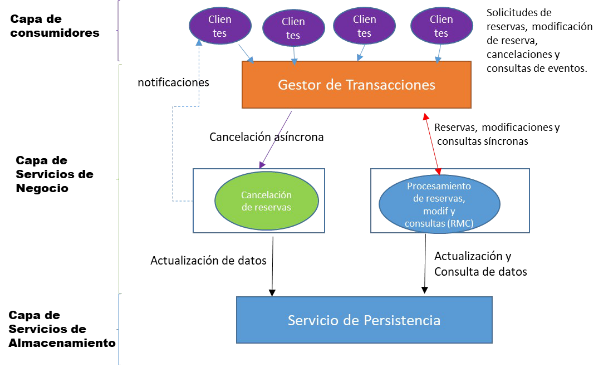
\includegraphics[width=0.7\textwidth]{Images/Modelo de capas sistema.png}
		\caption{Modelo arquitectónico de 3 capas del sistema}
		\label{fig:layers_model}
	\end{figure}
	
	La \textbf{capa de consumidores} se encarga de pasarle solicitudes y peticiones de los clientes al gestor de transacciones. Cada cliente puede hacer peticiones de reservas, modificación, consulta, y cancelación de reserva.
	
	La \textbf{capa de servicios} tiene dos procesos distintos. El \textit{gestor de transacciones} enruta las peticiones del sistema a su canal sincrono que se encarga de las solicitudes de reserva, modificación, y consultas mediante el proceso RMC y se comunicara con las demas capas mediantes el patrón REQ/ROUTER; o al canal asincrono, que usando el servicio de \textit{cancelación de reservas} y mediante el patrón PUSH/PULL se encarga de las solicitudes de cancelación pues estas no requieren notificar al cliente.
	
	Finalmente la \textbf{capa de almacenamiento} se encargara de garantizar la persistencia de las reservas de todo el sistema, esto lo hara mediante operaciones CRUD hacia una base de datos Postgress SQL.
	
	
	\subsection{Modelo de Interacción}
	\label{sec:models_exch}
	
	En este proyecto se integran tanto modelos síncronos como asíncronos. 
	En cuanto al modelo síncrono, se utiliza cuando los clientes quieren realizar reservas, modificaciones o consultas, estas solicitudes son recibidas por el gestor de transacciones el cual las enruta hacia el servicio RMC, en donde este solicita y aguarda la respuesta de la capa de almacenamiento, hasta que no suceda todo este proceso el cliente no recibe una confirmación. El patrón de comunicación que vamos a usar va a ser \textbf{request-router}, se escoge este ya que nos permite tener varias solicitudes al mismo tiempo, teniendo en cuenta que el request en este caso serían los clientes y el router seria el gestor de transacciones, estos se comunican mediante sockets y se le establece a cada solicitud un identificador único para su correcta respuesta.
	El modelo asíncrono se va a usar cuando los clientes quieran cancelar una reservación, es decir, entre el gestor de transacciones y el servicio de cancelación, el gestor acepta la cancelación y le da una respuesta inmediata al cliente; se va a realizar un patrón push/pull mediante pipeline ya que este incorpora un balanceador de cargas round robin el cual nos va a ayudar más adelante para la escalabilidad.
	
	\subsection{Modelo de Fallos}
	\label{sec:models_fail}
	Como se debe esperar que el gestor de transacciones o el RMC (Servicio que procesa reservas, modificaciones y consultas) fallen, planteamos un fallo de tipo fail-stop en donde un proceso falla pero los demás se dan cuenta del fallo, esto supone un problema grave ya que se requiere garantizar transparencia con los clientes dado que falle uno de los servicios más importantes como el gestor de transacciones o un servicio que hace varias funciones como lo es el RMC. En el peor de los casos el GT o el RMC presentarian un crash, sin embargo más adelante se verá nuestra propuesta para tratar la tolerancia a estos fallos.
	
	
	
	\subsection{Modelo de Seguridad}
	\label{sec:models_secu}
	La seguridad es un pilar importante en nuestro sistema; la confidencialidad e integridad son vulnerables debido a que se utiliza la libreria ZeroMQ por lo que si este canal no es asegurado los mensajes viajarian en texto plano permitiendo que un atacante pueda interceptar los datos. La disponibilidad se puede llegar a ver afectada si el gestor de transacciones recibe muchas DoS, lo cual podría llegar a saturarlo.
	
	
	\section{Diseño del Sistema}
	\label{sec:base_arch}
	
	Para comprender mejor el sistema se realizaron 4 diagramas de distintas vistas del sistema, vistas estáticas que permiten ver la estructura física y lógica del SRB junto con la forma en la que este funcionara internamente, y una vista dinámica que permite ver el comportamiento del SRB. 
	
	\subsection{Diagrama de Componentes}
	\begin{figure}[H]
		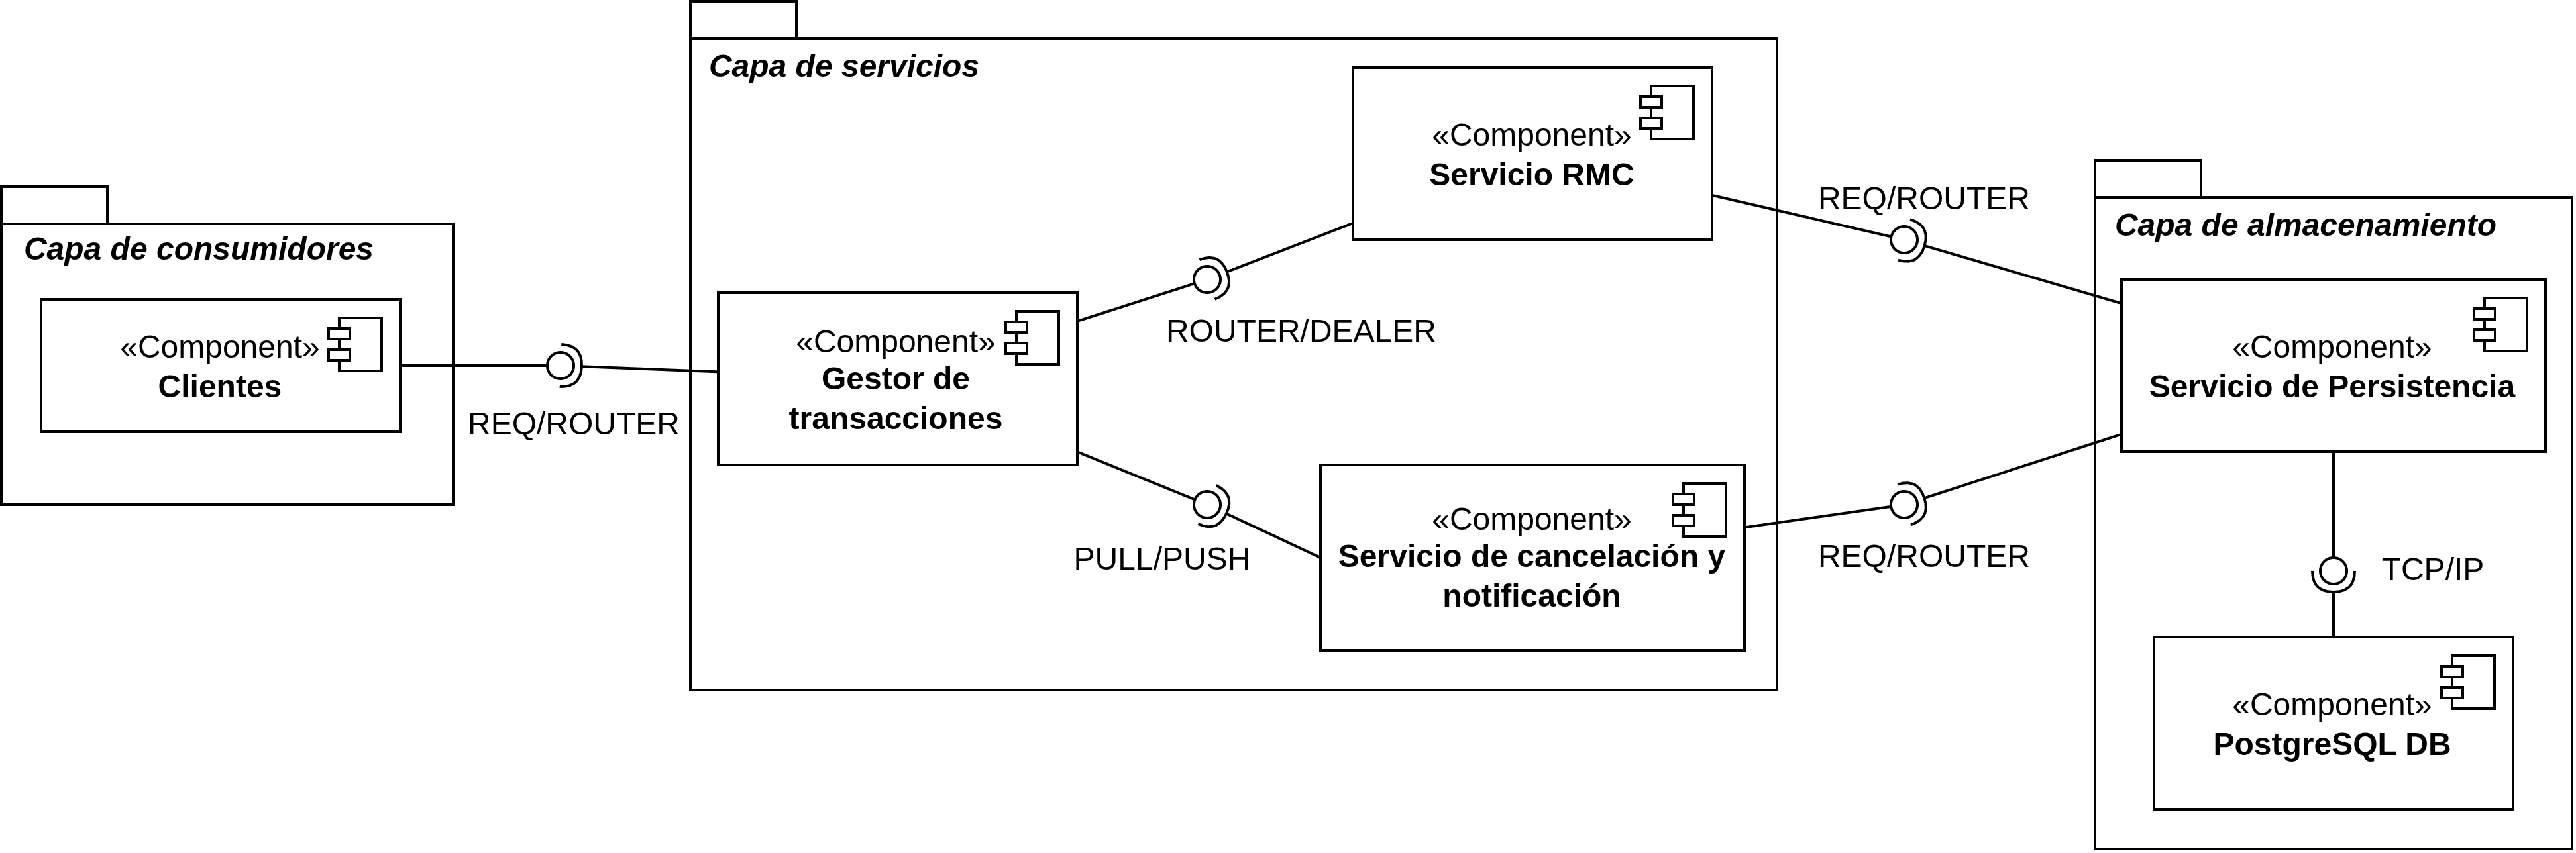
\includegraphics[width=1\textwidth]{Images/Diagrama de Componentes.png}
		\caption{Diagrama de componentes del SRB}
		\label{fig:comp_diagram}
	\end{figure}
	Este diagrama busca obtener una visualización más acertada sobre como trabajan los componentes entre sí y cuales son los protocolos que se usan para dicha comunicación.
	La mayor parte de las comunicaciones se hacen con el patrón REQ/ROUTER porque nos pareció una solución adecuada para este tipo de sistema. Por otro lado está la comunicación PULL/PUSH la cual se usa para mensajes asíncronos mediante un pipeline.
	Una última anotación es decidimos agregar un servicio llamado servicio de persistencia el cual se encarga de recibir las solicitudes de los servicios de cancelación y RMC para así poder interactuar con la base de datos, este es el único que lo puede hacer conectándose por TCP/IP.
	
	\subsection{Diagrama de Despliegue}
	
	\begin{figure}[H]
		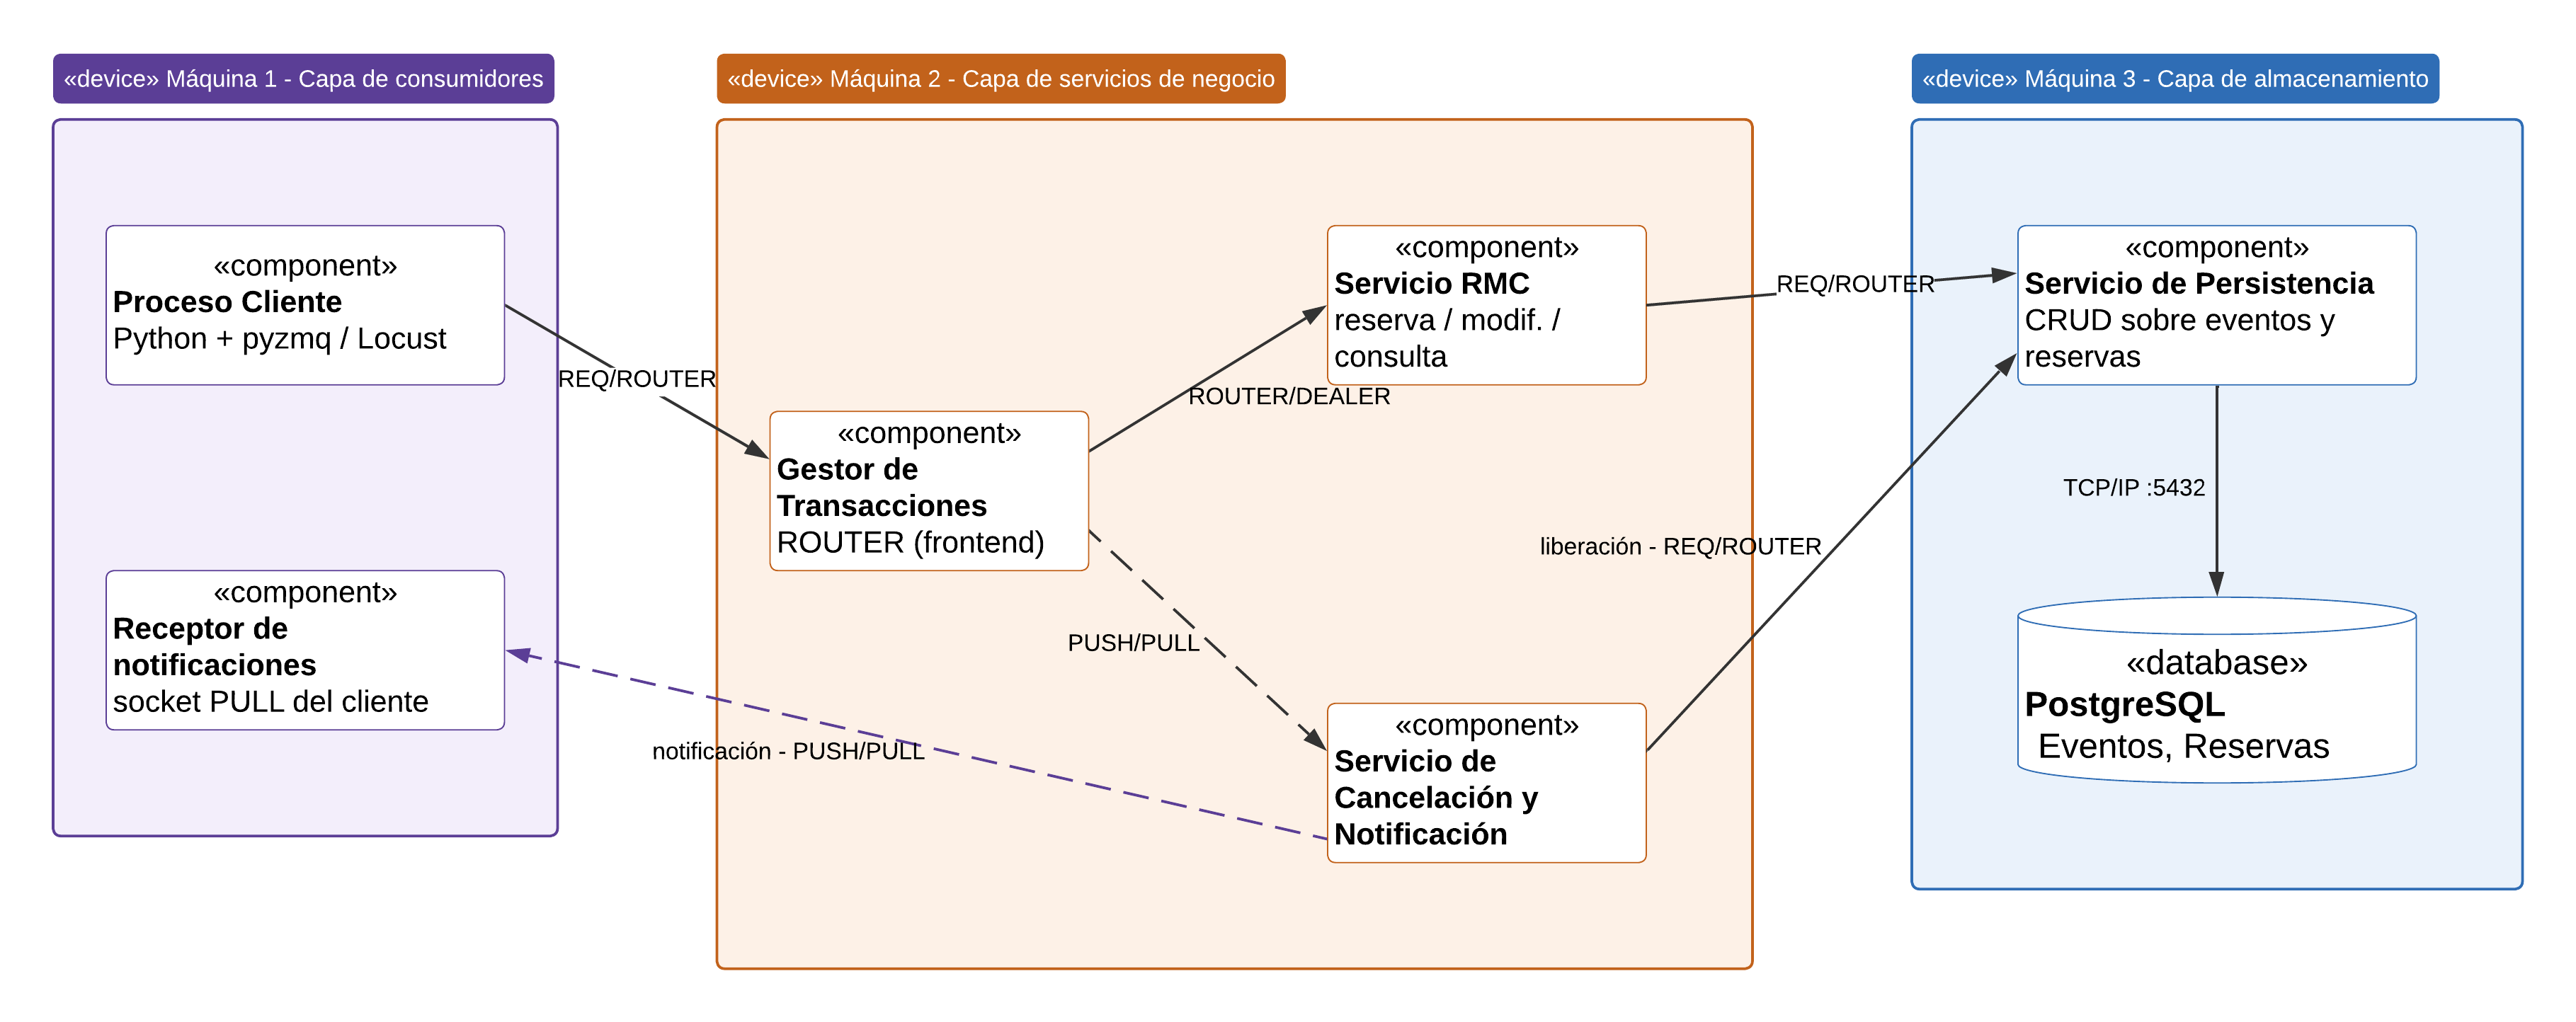
\includegraphics[width=1\textwidth]{Images/Diagrama de Despliegue.png}
		\caption{Diagrama de Despliegue del SRB}
		\label{fig:deploy_diagram}
	\end{figure}
	La figura~\ref{fig:deploy_diagram} muestra la distribución del sistema en tres máquinas, una por capa. En la primera se ejecutan los clientes, desarrollados en Python con pyzmq, y Locust para generar carga. Cada cliente cuenta además con un receptor PULL para recibir el resultado de sus cancelaciones.

    En la segunda máquina se ubican el Gestor de Transacciones, el servicio RMC y el servicio de Cancelación y Notificación. El gestor recibe las solicitudes y selecciona su destino: las consultas, reservas y modificaciones pasan al RMC, mientras que las cancelaciones se envían por PUSH/PULL para procesarlas sin mantener al cliente esperando el resultado final. La figura representa ROUTER/DEALER en la comunicación entre el gestor y el RMC.

    La tercera máquina contiene el servicio de persistencia y PostgreSQL, al que se accede por el puerto 5432. El RMC y el servicio de cancelación solicitan los cambios a persistencia; los clientes no acceden directamente a la base. La notificación final vuelve desde cancelaciones al receptor del cliente, utilizando la dirección que este proporciona. Así, el diagrama permite identificar tanto la ubicación de los procesos como las conexiones necesarias entre las máquinas.
	
	\subsection{Diagrama de Clases}
	
	\begin{figure}[H]
		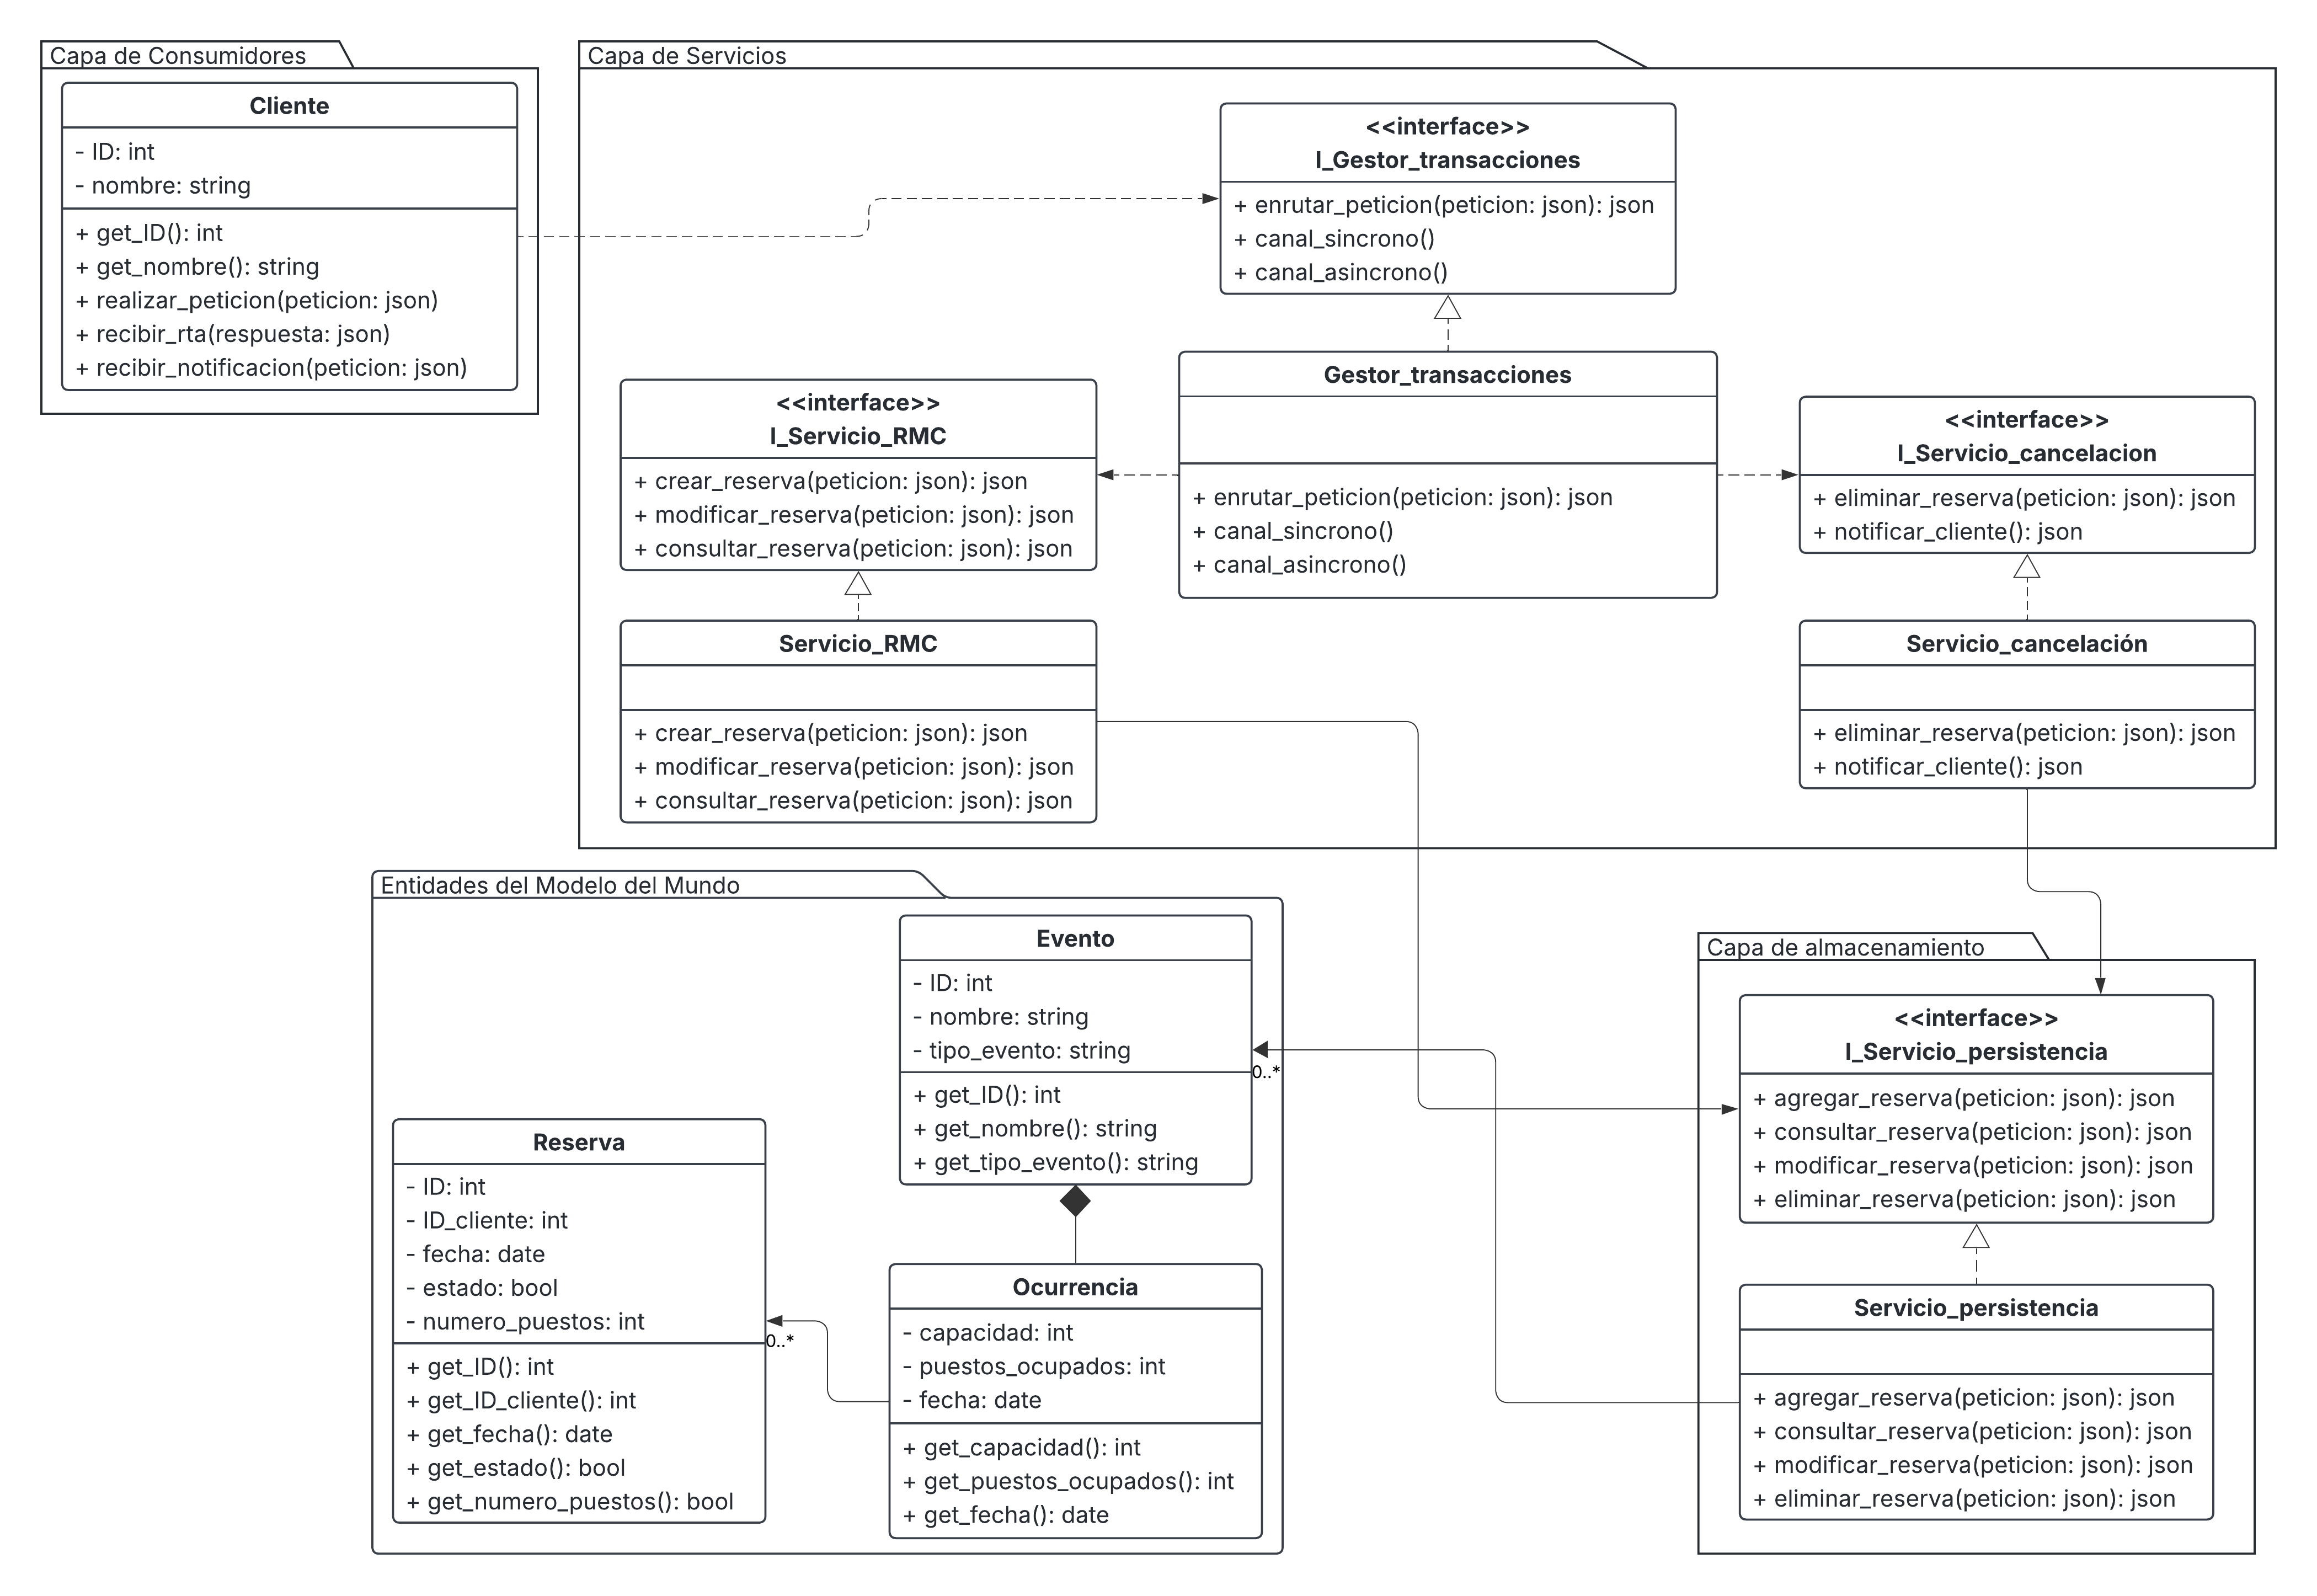
\includegraphics[width=1\textwidth]{Images/Diagrama de Clases.png}
		\caption{Diagrama de clases del SRB}
		\label{fig:class_diagram}
	\end{figure}
	La figura~\ref{fig:class_diagram} organiza las entidades del negocio y las responsabilidades de los servicios. \textbf{Evento} identifica la actividad mediante su nombre y tipo; \textbf{Ocurrencia} representa una fecha concreta de esa actividad y registra su capacidad y puestos ocupados. Esta separación permite que un mismo evento se realice en distintas fechas, cada una con su propia disponibilidad. \textbf{Reserva} contiene el identificador, la fecha, el estado y la cantidad de puestos solicitados, mientras que \textbf{Cliente} identifica a quien realiza las peticiones.

    En la capa de servicios, \textbf{GestorTransacciones} selecciona el canal de atención. \textbf{ServicioRMC} reúne las operaciones de creación, modificación y consulta, y \textbf{ServicioCancelación} recibe las solicitudes para eliminar una reserva. Ambos utilizan \textbf{ServicioPersistencia}, que concentra las operaciones sobre los datos y se comunica con \textbf{DataBase}. Las relaciones muestran qué entidades y servicios colaboran; no representan acceso directo de los clientes a PostgreSQL. El diagrama expresa el diseño lógico propuesto, y la consulta de eventos por mes se detalla en la secuencia siguiente.
	
	\subsection{Diagrama de Secuencia}
	
	\begin{figure}[H]
		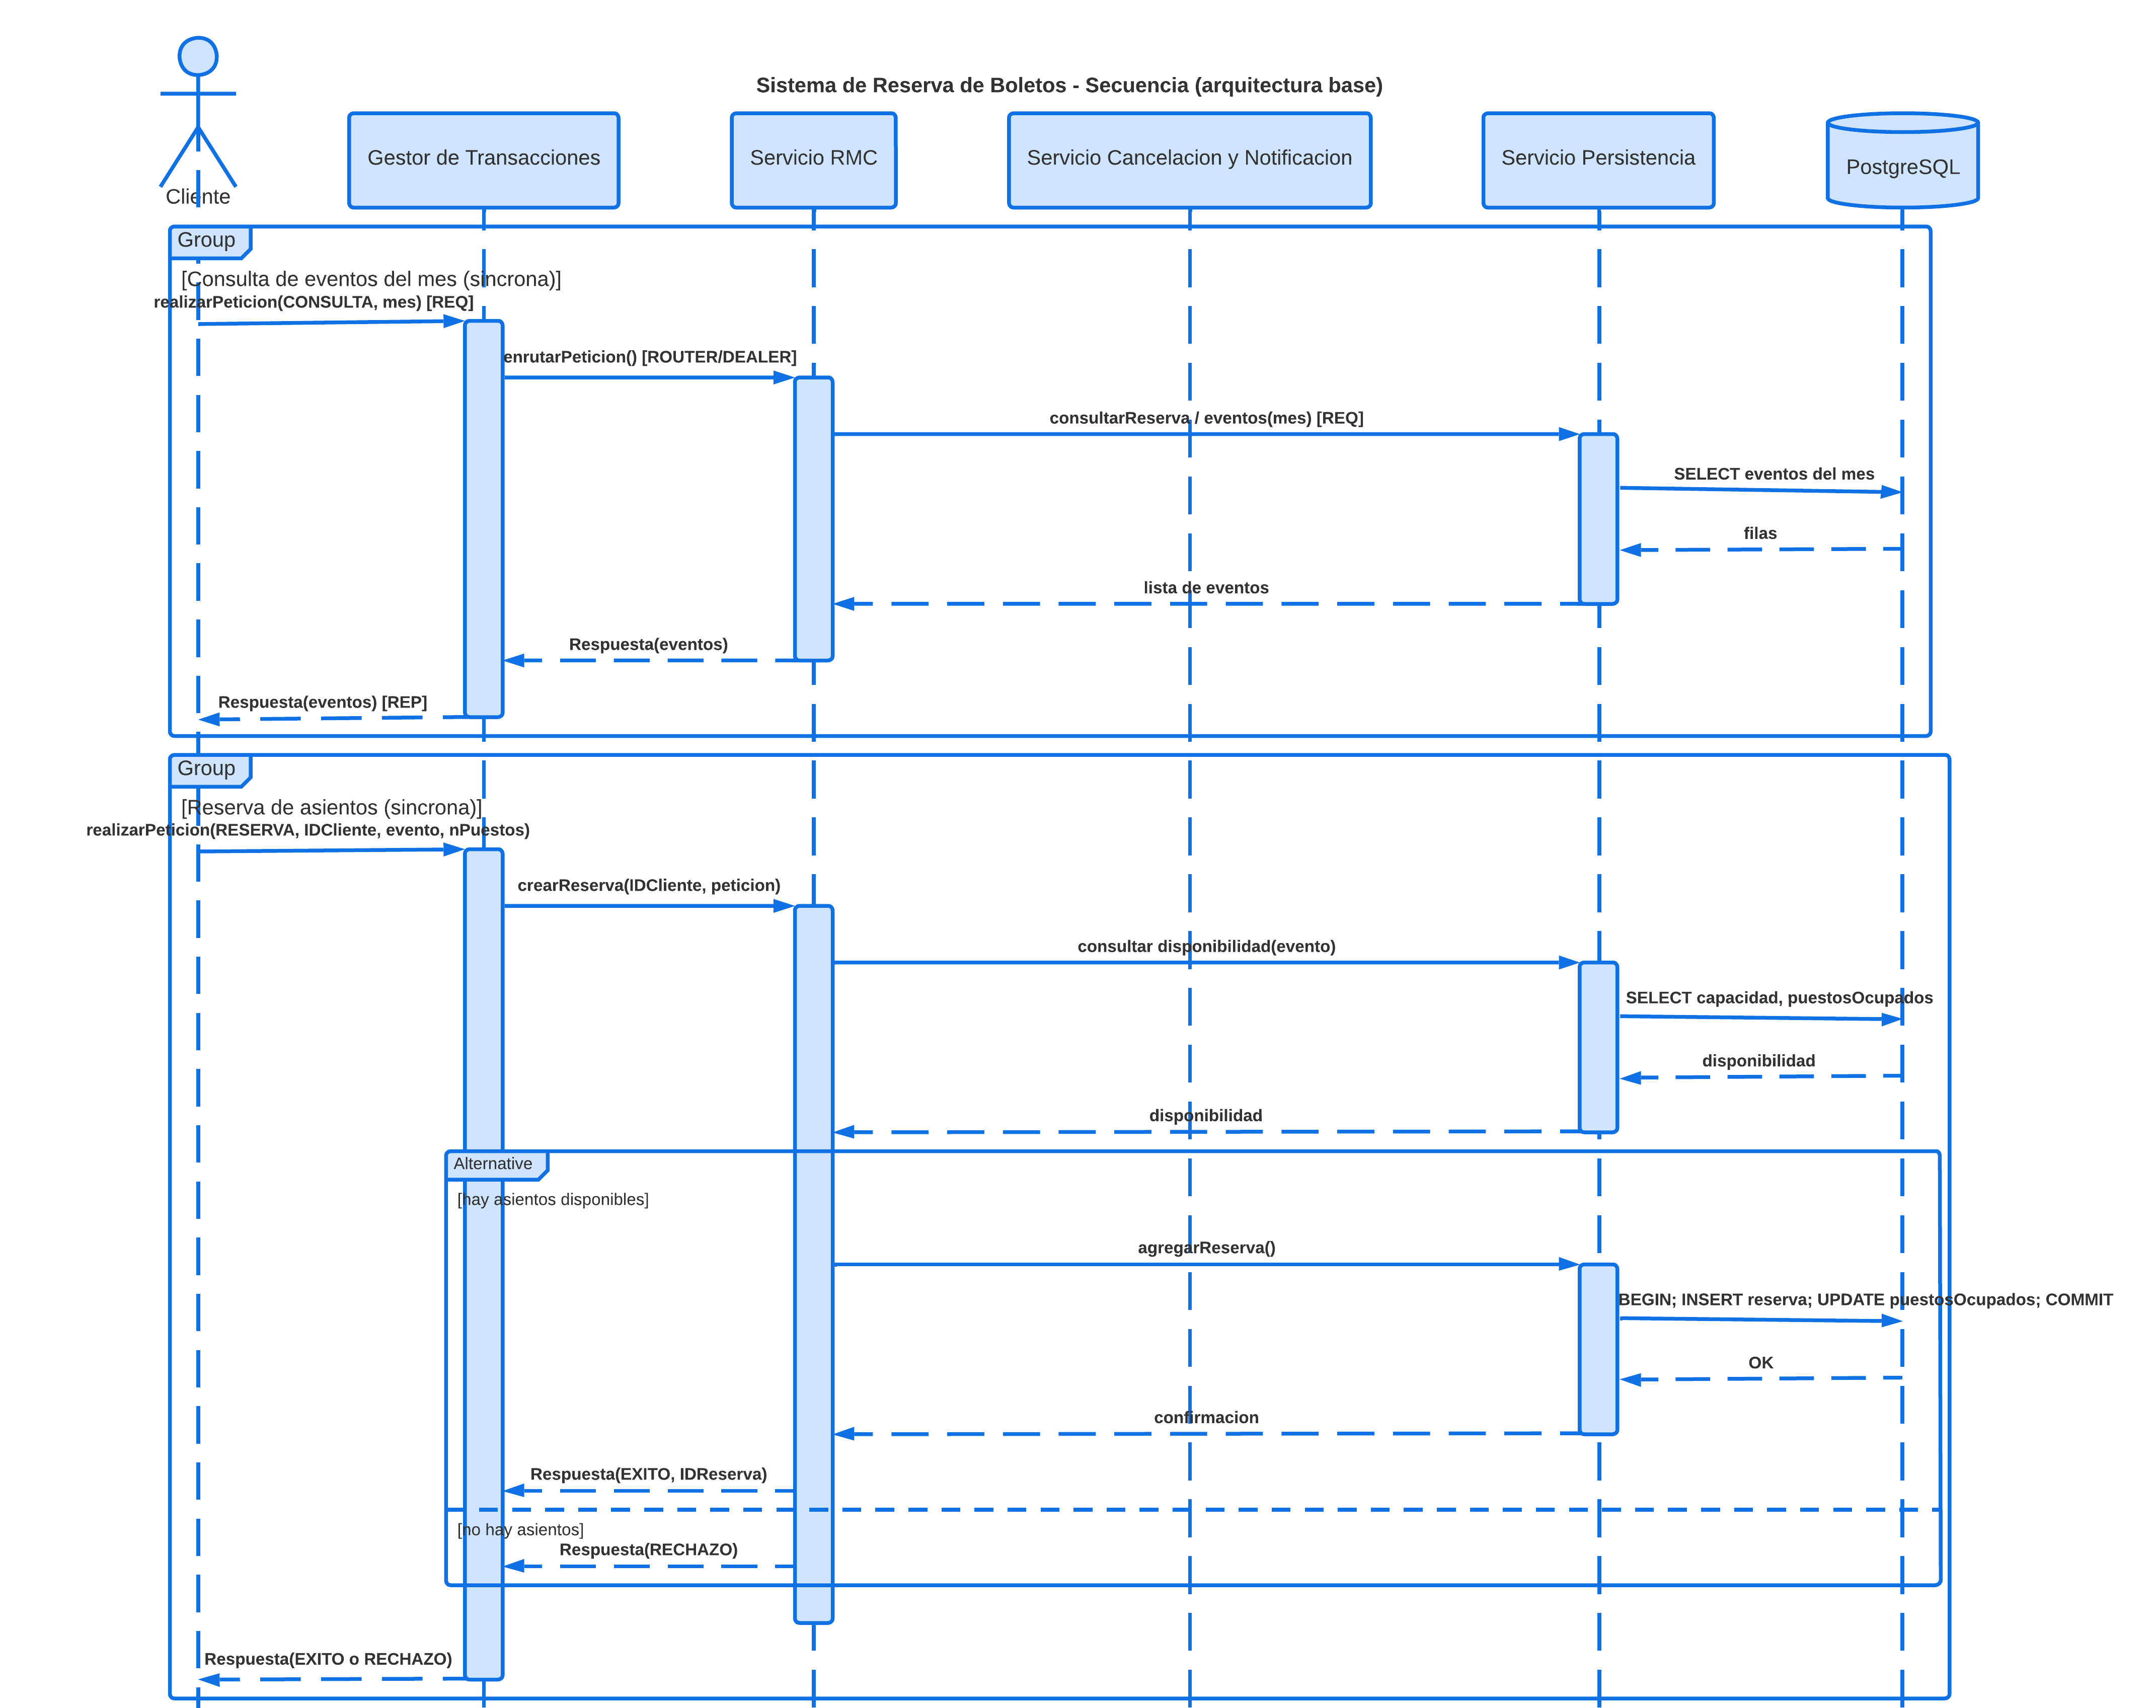
\includegraphics[width=1\textwidth]{Images/Diagrama de Secuencia - 1.png}
		\caption{Secuencia de consulta y reserva del SRB}
		\label{fig:seq_diagram1}
	\end{figure}
	La figura~\ref{fig:seq_diagram1} se lee de arriba hacia abajo y presenta dos operaciones síncronas. En la \textbf{consulta}, el cliente indica el mes al gestor, este remite la petición al RMC y persistencia obtiene los eventos de PostgreSQL. La lista regresa por el mismo recorrido hasta el cliente.

    En la \textbf{reserva}, el cliente envía su identificación, el evento y la cantidad de puestos. El RMC solicita la disponibilidad y, si existe cupo, pide a persistencia crear la reserva y actualizar la ocupación. El bloque de alternativas distingue la confirmación del rechazo por falta de asientos. La respuesta exitosa, que incluye el identificador de reserva, se devuelve después del \texttt{COMMIT}. Aunque la figura separa la consulta de disponibilidad de la escritura, la implementación deberá volver a comprobar el cupo dentro de la transacción para evitar que solicitudes simultáneas reserven los mismos puestos.
	
	\begin{figure}[H]
		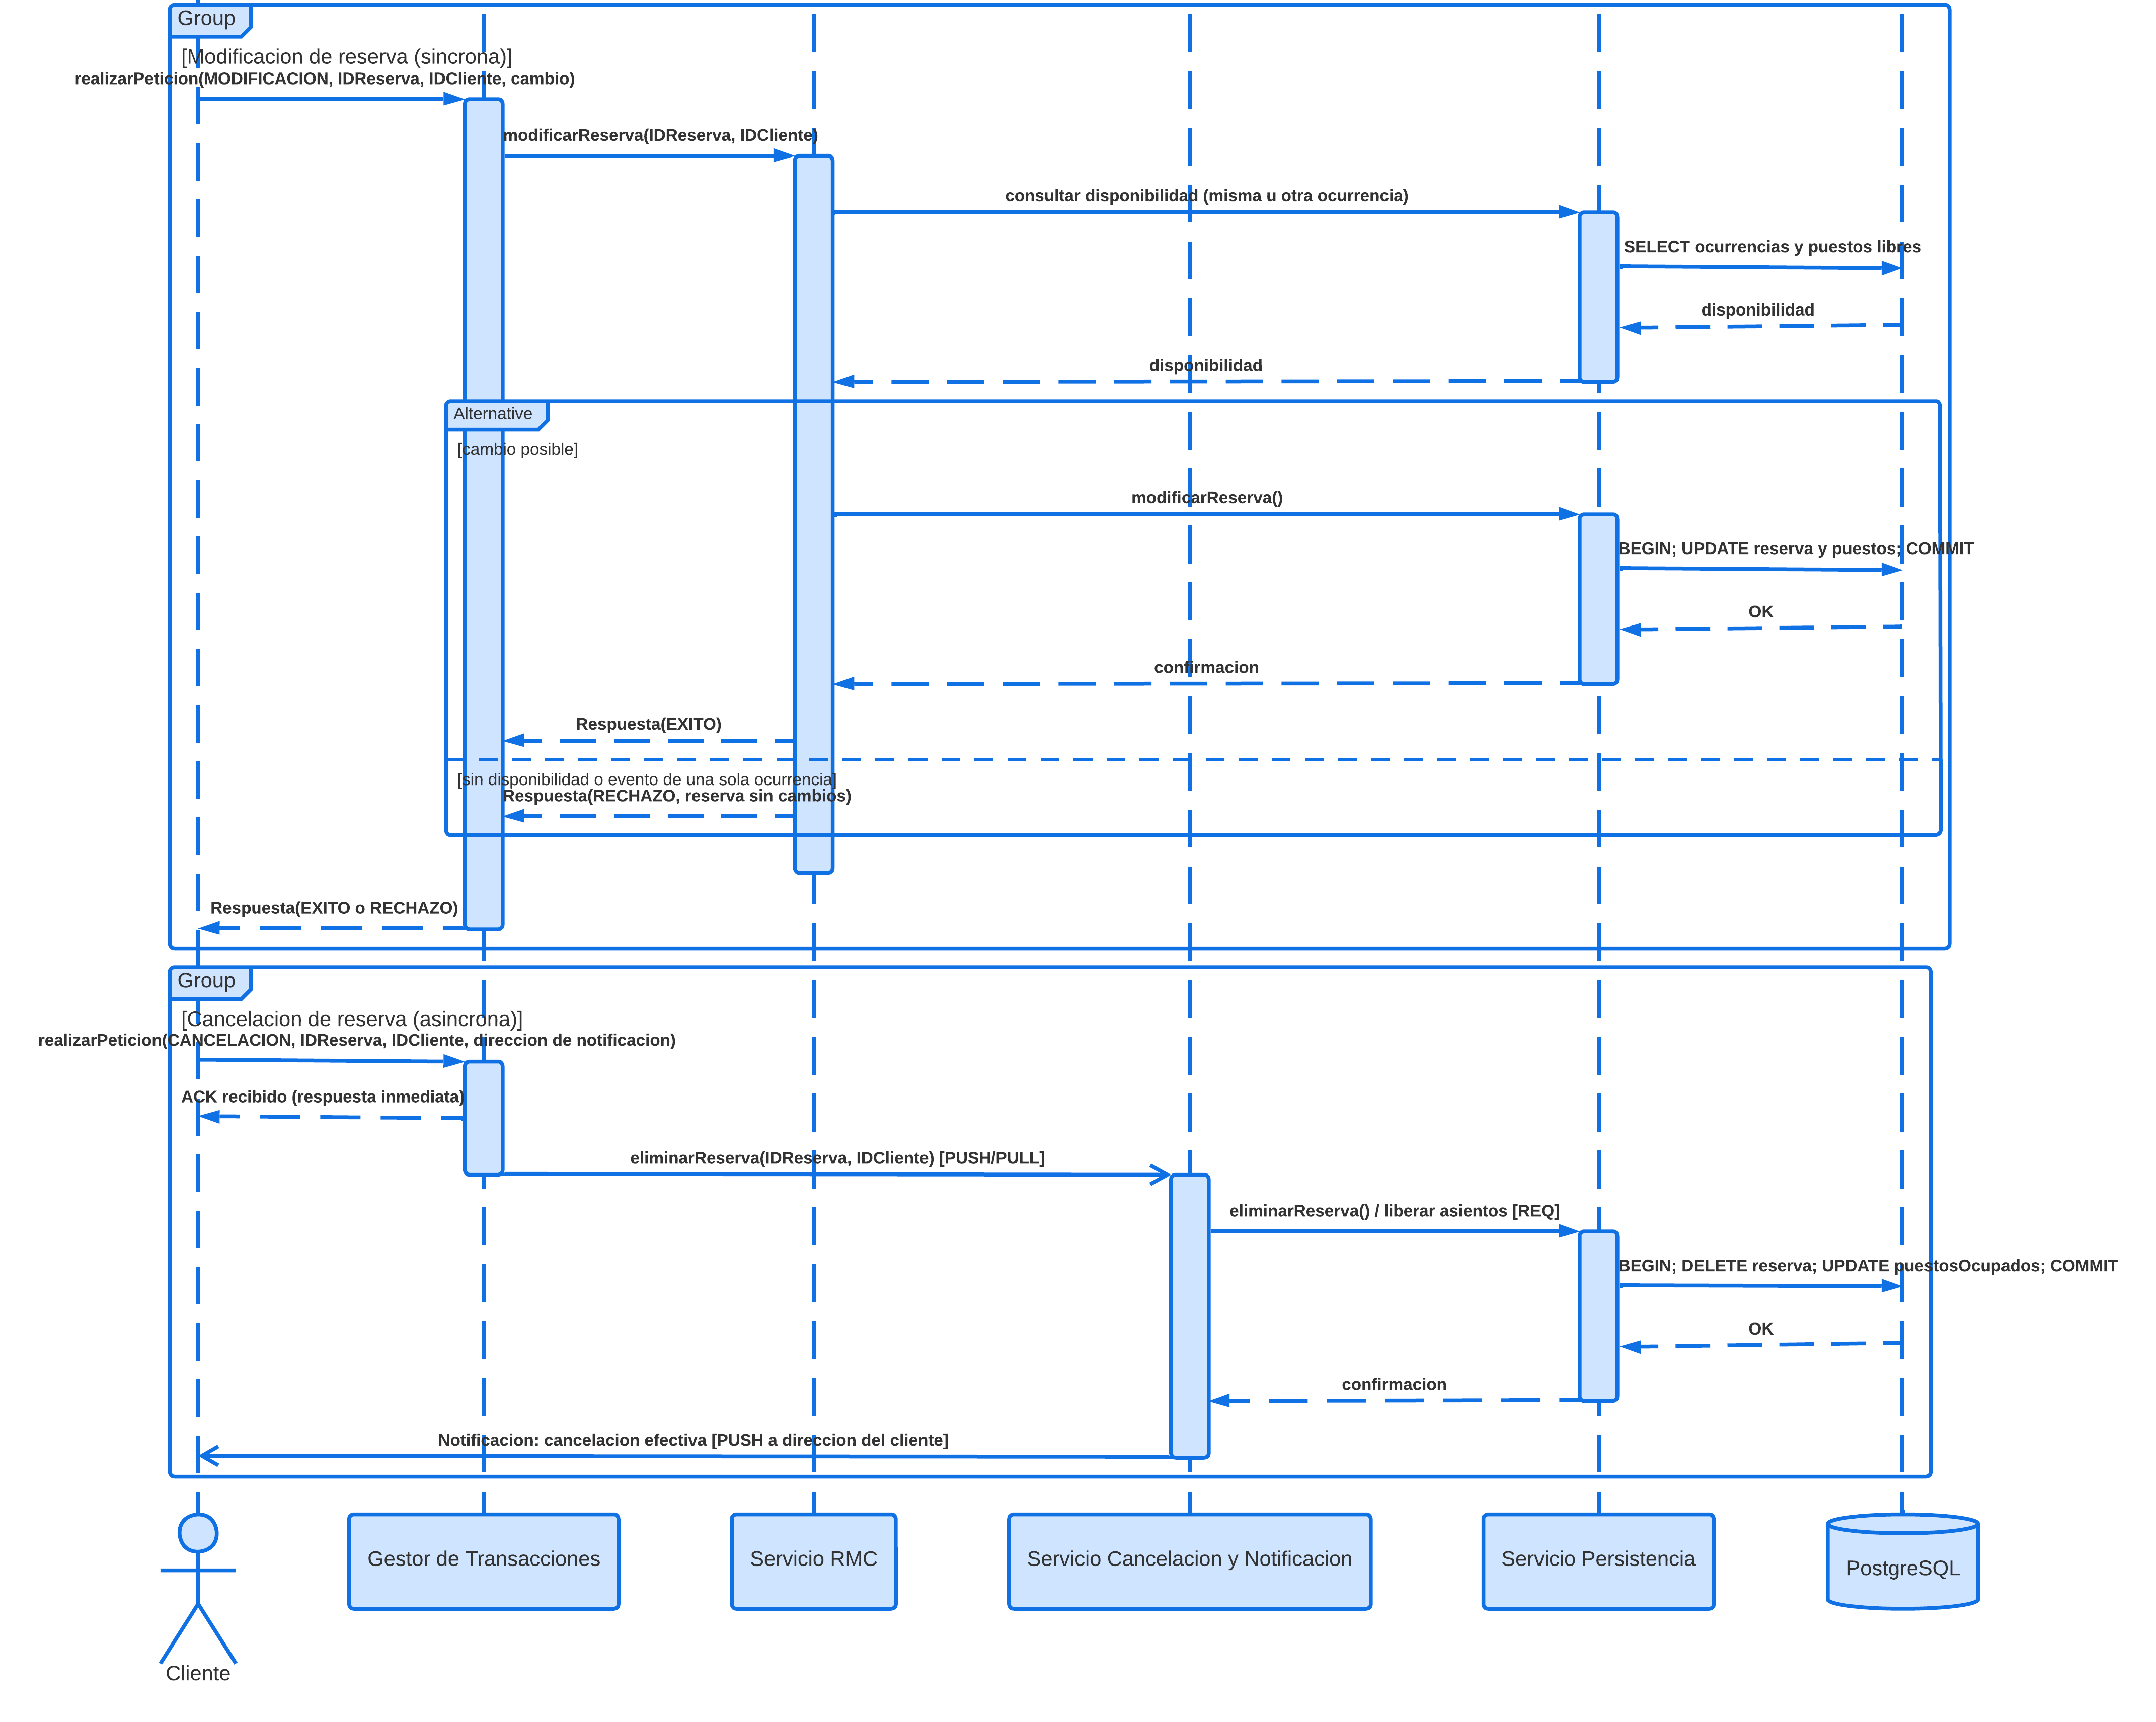
\includegraphics[width=1\textwidth]{Images/Diagrama de Secuencia - 2.png}
		\caption{Secuencia de modificación y cancelación del SRB}
		\label{fig:seq_diagram2}
	\end{figure}
	La figura~\ref{fig:seq_diagram2} continúa con la \textbf{modificación}. El cliente identifica su reserva y el cambio solicitado; el RMC comprueba la disponibilidad mediante persistencia. Si el cambio es válido, se actualizan la reserva y la ocupación en una misma transacción. Si no es posible, se devuelve un rechazo y se conserva la reserva original. El cambio de fecha solo admite otra ocurrencia del mismo evento y mes, manteniendo la cantidad de puestos. Un evento con una sola ocurrencia sí permite modificar esa cantidad, aunque no cambiar de fecha.

    En la \textbf{cancelación}, el cliente incluye la dirección donde recibirá la notificación. El gestor devuelve una aceptación inmediata y envía el trabajo al servicio de cancelación mediante PUSH/PULL. Este solicita a persistencia eliminar la reserva y liberar los asientos. Solo después de confirmar el cambio en PostgreSQL se notifica directamente al cliente. Por tanto, la aceptación inicial indica que la solicitud fue recibida; la notificación posterior confirma que la cancelación se hizo efectiva. El envío final debe dirigirse al receptor de ese cliente, evitando repartir las notificaciones entre clientes distintos.
	
	\section{Estrategia de Escalabilidad y Tolerancia a Fallos}
	\label{sec:scalability}
	La estrategia de escalabilidad se fundamenta en hacer escalamiento horizontal en la capa que lo requiera, donde cada maquina sera una capa distina y cada capa tendra un contenedor por proceso. Para los servicios de negocio sin estado como RMC y Cancelaciones, la capacidad se incrementa instanciando dinámicamente nuevos contenedores cuyo tráfico es distribuido por el Gestor de Transacciones mediante el patron ROUTER-DEALER con ZeroMQ. Por su parte, la capa de persistencia con estado en PostgreSQL se escala mediante un esquema de replicación de base de datos, garantizando alto rendimiento en transacciones por minuto, aislamiento de recursos y alta disponibilidad.
	
	El manejo de fallos usara dos estrategias, para los fallos fail-stop en RMC se implementaran time outs, estos confirman si el proceso murio o no, en cancelaciones se esperara que el proceso envie "señales de vida" cada cierto tiempo pues dependiendo de esa señal el detector determinara si el proceso se considera como muerto o no. En caso de que un proceso especifico falle, sera reemplazado por una copia del mismo para garantizar la transparencia de fallos.

	\section{Protocolo de Pruebas de la entrega final}
	\label{sec:protocol}
    Se ejecutarán las siguientes pruebas sobre el sistema final. Cada caso registrará entradas, estado inicial, resultado obtenido y evidencia, para contrastarlos con el resultado esperado.

    \begin{table}[H]
        \centering
        \footnotesize
        \renewcommand{\arraystretch}{1.15}
        \begin{tabular}{@{}p{\dimexpr0.18\linewidth-2\tabcolsep\relax}p{\dimexpr0.42\linewidth-2\tabcolsep\relax}p{\dimexpr0.40\linewidth-2\tabcolsep\relax}@{}}
            \toprule
            \textbf{Tipo de prueba} & \textbf{Procedimiento} & \textbf{Resultado esperado} \\
            \midrule
            Unitarias y límites & Validar meses, cantidades, identificadores y disponibilidad, incluyendo cupo exacto e insuficiente. & Entradas válidas aceptadas; entradas inválidas rechazadas sin cambios en los datos. \\
            Integración & Recorrer cliente--GT--RMC--persistencia y verificar solicitudes y respuestas. & Respuesta al cliente correcto y confirmación de escritura únicamente después de persistir el cambio. \\
            Funcionales & Consultar, reservar y modificar cantidad o fecha. Probar cambios sin cupo y fechas no permitidas. & Consultas correctas; cambios de fecha dentro del mismo evento y mes, conservando la cantidad. Ante rechazo, reserva original intacta. \\
            Cancelación asíncrona & Solicitar cancelaciones con varios clientes conectados y comprobar las notificaciones. & Aceptación sin esperar la cancelación efectiva; liberación una sola vez y notificación posterior al cliente solicitante. \\
            Concurrencia & Veinte clientes solicitan un asiento cuando quedan diez disponibles. & Diez confirmaciones y diez rechazos, sin sobreventa; libres más ocupados igual a la capacidad. \\
            Fallos y persistencia & Detener GT/RMC antes y después de guardar cambios; sustituir procesos y reintentar con el mismo ID. Reiniciar servicios. & Datos confirmados conservados; continuación de operaciones pendientes sin reiniciar el trabajo del cliente ni duplicar efectos. \\
            Seguridad & Enviar mensajes malformados e intentar modificar o cancelar reservas ajenas. & Rechazo sin cambios no autorizados; el servicio continúa atendiendo solicitudes válidas. \\
            Rendimiento y escalabilidad & Comparar arquitectura base y escalable con Locust en los escenarios de 3, 5 y 8 clientes. & Medición de promedio y desviación de latencias de consulta y reserva, y TPM por operación en el GT; comparación mediante tablas y gráficos. \\
            Estrés y duración & Aumentar la carga y mantener una ejecución prolongada. & Identificar saturación, acumulación de pendientes y crecimiento del consumo de recursos. \\
            Despliegue, aceptación y regresión & Ejecutar el README en tres máquinas, aplicar los casos del profesor y repetirlos tras cambios relevantes. & Comunicación entre capas y notificaciones operativas; estado final de la BD acorde con cada caso y funciones previas conservadas. \\
            \bottomrule
        \end{tabular}
        \caption{Protocolo de pruebas previsto para la entrega final.}
        \label{tab:protocol}
    \end{table}

    Las pruebas de rendimiento durarán 2--3 minutos, con al menos 20 solicitudes por minuto por cliente y mezcla parametrizable. En los escenarios de 3, 5 y 8 clientes, respectivamente 2, 3 y 4 solo consultarán; los restantes consultarán y reservarán en el primero, y reservarán y modificarán en los otros dos. Se mantendrán datos iniciales y condiciones equivalentes entre arquitecturas. Se conservarán reportes, logs, estados de la BD y CSV, separando éxitos, rechazos y errores técnicos.
	
	\section{Estrategia de obtención de métricas y carga de los clientes}
	\label{sec:testing}
	% Define the testing protocol for the final delivery.
	% Specify tools/methods for client load generation (Locust or JMeter).
	La herramienta que vamos a usar es \textbf{Locust} ya que permite ver los tiempos de respuesta y los errores en tiempo real, además su lenguaje es en python y se puede ejecutar en varias máquinas, lo que nos asegura medir de forma óptima la escalabilidad.
	
\end{document}
